\documentclass[conference,compsoc]{IEEEtran}

%%%%%%%%%%%%%%%%%%%%%%%%%%%%%%%%%

%Linguagem e acentuação\textsl{}
\usepackage[utf8]{inputenc}
\usepackage[T1]{fontenc}
\usepackage{lmodern}

%Imagens
\usepackage{graphicx}

%Tabelas
\usepackage{multicol}
\usepackage{booktabs}
\usepackage{multirow}

%Algoritmo
\usepackage[english, ruled, lined, linesnumbered]{algorithm2e}
\SetKwInOut{Input}{Input}
\SetKwInOut{Output}{Output}


%Gramática
\usepackage[nounderscore]{syntax}
\usepackage{amsmath}
\grammarindent 80pt

%Renomear TABLE para TABELA
%\renewcommand{\tablename}{TABELA.}
%\renewcommand{\refname}{Referências}
%%%%%%%%%%%%%%%%%%%%%%%%%%%%%%%%%

\begin{document}
	
\title{A grammatical evolution approach to generate clustering algorithms}


\author{
Vidal D. da Fontoura\\
Universidade Federal do Paraná\\
vidalfontoura16@gmail.com
\and
Ricardo H. R. de Lima\\
Universidade Federal do Paraná\\
ricardo.hrlima@gmail.com
}


% make the title area
\maketitle

\begin{abstract}
	
	% Nowadays, there is an increase of data generated everywhere and is becoming crucial to analyze and extract the hidden information. 
	
	Nowadays, with the increasing amount of data generated, clustering algorithms are fundamental to extract hidden and useful information. They group similar data and allow a better interpretation. Each obtained group has objects that are close to each other considering its characteristics, and are different from objects from other groups. However, such algorithms depend on many parameters and are domain dependent, hindering their application. In this context, the field of hyper-heuristics raises as an alternative by allowing the generation of a custom clustering algorithm, and to contribute to this research subject, this work proposes the automatic design of clustering algorithms by using a hyper-heuristic based on Grammatical Evolution. Grammatical Evolution is a type of Genetic Programming that uses a Backus-Naur Form Grammar to evolve a population of computer programs to solve a problem. The proposed approach includes a grammar that captures the main features of clustering algorithms and a fitnes function based on the silloutte index. It is implemented by the algorithm GE-Clust. Such algorithm was evaluated in different bases from the UCI repository and compared to the K-means algorithm. The approach  shows promising results  and advantages. For example, there is no need to configure the number of clusters.
	
\end{abstract}

% no keywords

\IEEEpeerreviewmaketitle

\section{Introduction}

Modern methods of data collection have allowed gathering a huge quantity of data. Therefore, there is an increasing demand for grouping and filtering important data and extract useful information from the collected data~\cite{ahalya2015data}, and as a consequence, a crescent research interest in the area of clustering algorithms. Clustering is the unsupervised learning of patterns (observations, data items, or feature vectors) into groups (clusters)~\cite{jain1988algorithms}. Clustering approach applications have increased in various areas of Artificial Intelligence, data mining, image recognition, data statistics, etc. The main goal is to determine the intrinsic grouping in a set of unlabeled data~\cite{ahalya2015data}.

The main problem in the application of clustering methods is that the algorithms need many parameters that are domain dependent, hindering their application. In this sense, the field of hyper-heuristics raises as an alternative by allowing the generation of a custom algorithm. Hyper-heuristics is a field of study that aims automatically creating novel algorithms designed to perform better on certain classes of problems than would a general algorithm modified by hand for that purpose~\cite{harris2015comparison}. The automatic design of the algorithms using Hyper-heuristics is  often done through the use of genetic programming techniques. Genetic Programming (GP) is a type of Evolutionary Algorithm (EA) that has raised interest over the years. GP is a domain-independent method that genetically breeds a population of computer programs to solve a problem, it evolves the solutions by the application of selection, mutation and crossover operators~\cite{poli2014genetic}. The GP provides a way to automate one of the most expensive and time-consuming aspects of the software engineering process: the production of the code itself~\cite{langdon2013optimising}. The GP algorithms are responsible for selection of individual parts (functions, routines, pieces of code) to build an algorithm and then evaluate it in order to search for a design that best solve a certain type of problem.

Deeper in the idea of evolving computer programs, one of the used approaches in Genetic Programming is the Grammatical Evolution (GE), where a BNF (Backus-Naur Form) grammar is used to generate sentences for a given language, theses sentences are mapped into  computer programs that are evaluated by the algorithm. Finally, the generated algorithm is executed and its performance is used as feedback for the evolutionary process.

Existing approaches for evolving clustering algorithm does not use GE. Some works like \cite{ahn2011genetic, xie2006population, boric2007genetic} make use tree-based GP for Clustering. Although \cite{harris2015comparison} say that GE and GP have the same search space, for some problems the use of GE could make easier to work with it. Working with a tree-representation for the individuals is more difficult than deal with an integer vector.


Falta uma ligacao com a motivação

%S good não está legal.... podemos até usar mas precisamos dizer como medimos o quao good sao...

In this paper we propose an approach for automatic design of clustering algorithms by applying Grammatical Evolution. The hypothesis that guides our work is that such approach is capable to generate clustering algorithms that can classify data as well as well-know algorithms for that purpose, and . The main advantage is to reduce the effort required to the algorithm design. To this end, we first define a grammar that captures the main clustering algorithm features. Then, algorithms are generated for different bases of the UCI repository~\cite{}. and finally, the obtained clustering algorithms are compared to K-means~\cite{} considering some indicators, such as ...



This paper is organized as follows. Section~\ref{sec:theoretical_foudation} reviews some topics that are important for the full understanding of the paper. Section~\ref{sec:methodology} introduces our approach,  describes the grammar proposed for the design of the algorithms and how the algorithms are generated using GE. Section~\ref{sec:experiments} describes how the conducted experiments,  presents the obtained results and shows the comparison to K-means algorithm. Finally, the Section~\ref{sec:conclusion} concludes the paper and shows future research directions.


%%%%%%%%%%%%%%%%%%%%%%%%%%%%%%%%%%%%%%%%%%%%%%%%%%%%%%%%%%%%%%%%%%%%%%%%%%

\section{Theoretical Foundation} \label{sec:theoretical_foudation}

This section presents background and some important concepts used in our work. First, a review of genetic programming is presented. Then, grammatical evolution is addressed, i.e., we show how the grammar supports the generation of programs, and how to choose and map the individuals into programs. Moreover, the clustering problem is described.


\subsection{Genetic Programming}

Genetic Programming (GP) is a systematic method for getting computers to automatically solve a problem from a high-level statement of what need to be done~\cite{koza2005genetic}. Having a similar behavior to Genetic Algorithms (GAs), GP iteratively evolves a population of computer programs, applying the selection, crossover and mutation operators, in order to improve their fitness, and increase the chances of an individual being part of future generations.

Different from AGs, GP works with computer programs, and because of this, the use of a different structure for individual's representation is needed. There are many ways to represent individuals, some of the most used are: the syntax tree and linear representation.

The original formulation of genetic programming was done with a tree representation. Here, each node on the tree is a function that takes its children as inputs and sends its output to its parent. Each sub-tree is a complete sub-program. However, there is no capacity for parts of the tree to be reused in a calculation (like in loops), which makes some things more difficult to be done~\cite{harris2015comparison}. 

%S Não entendi o parágrafo abaixo. quem é que produz os nos...

Grammatical evolution, a genetic programming variant, uses a genotype that represents a set of nodes, which are translated to a list of grammatical expansions that eventually produce other nodes (%SN???). 
This potentially allows the user to have more control over the search space, and also facilitates the use of multiple data types in the algorithm. The genotype is represented linearly but can be decoded into a tree for execution and evaluation. In terms of what can be represented, unless restricted in its grammar, this GP variant has the same power over the search space as the tree-based GP~\cite{harris2015comparison}.


\subsection{Grammatical Evolution} \label{subsection:grammaticalEvolution}

Grammatical evolution is a grammar based form of genetic programming. GE accomplishes the mapping process by combining a context free grammar (CFG) with a rule selection mechanism implemented using a genetic algorithm~\cite{byrne2015optimising}.

The main difference between GE and GP, is that in GP, both genotype and phenotype of the individual that is under evolution are derivation trees, whilst in GE, genotype and phenotype have different encoding structures. The genotype is represented as a linear string of codons (sequence of 8 bits) of variable size, which is then decoded into a vector of integers. The phenotype, which is the structure that defines fitness, is represented by a derivation tree (resulting from the application of a grammar)~\cite{cerri2013grammatical}. The clear distinction between the genotype and phenotype in GE allows the evolutionary process to be performed on the search space (variable length linear genotypic) without needing to tailor the diversity-generating operator to the nature of the phenotype~\cite{sabar2013grammatical}.

The grammar is a set of structural rules that define the composition of sentences for a given language. Grammatical rules provide a concise way of restricting a language while allowing endless variation through recursive application of the rules~\cite{byrne2015optimising}. The grammar is represented by Backus-Naur Form (BNF). The program is generated using an integer vector, where each codon (vector position) value, is used to determine which production rule in the BNF grammar will be used.

Figure~\ref{fig:grammar} shows a basic BNF (Backus-Naur Form) grammar, that can be used to generate simple math equations. In the group of terminal nodes, we have: +, -, *, /, as operations and x, y and z as variables. For the non-terminal nodes, we have: $<$op$>$, $<$expr$>$ and $<$var$>$.

\begin{figure}[!htb]
	\centering
	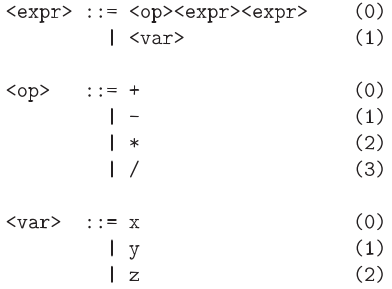
\includegraphics[scale=.6]{figures/grammar.png}
	\caption{Example of basic grammar.~\cite{ryan1998grammatical}}
	\label{fig:grammar}
\end{figure}



\begin{figure}[!htb]
	\centering
	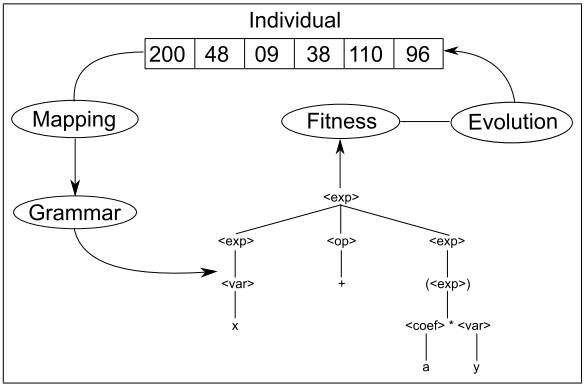
\includegraphics[scale=.4]{figures/ge_algo.png}
	\caption{Basic scheme for mapping process.~\cite{cerri2013grammatical}}
	\label{fig:ge_algo}
\end{figure}

A mapping process is needed to convert the bit string (genotype) into the derivation tree (phenotype), so the fitness can be evaluated. The mapping process is shown in Figure~\ref{fig:ge_algo}. Starting from the bit string or integer vector, each codon has its value used in the Equation~\ref{eq:map} to select a derivation rule from the grammar:

\begin{equation}\label{eq:map}
GR_i = int~~mod~~nr_i
\end{equation}

where $GR_i$ is the index of the grammar rule to be selected in non-terminal $i$, $int$ is the codon integer value and $nr_i$ is the number of rules available for derivation in non-terminal $i$. The operator $mod$ returns the remainder of the division between two numbers.


\subsection{Clustering}

The Clustering problem consists in partitioning a dataset into subgroups such that items belonging to the same group are more similar than those belonging to different groups~\cite{boric2007genetic}~\cite{ahalya2015data}. The application of clustering approaches has widely increased in the areas of Artificial Intelligence, pattern recognition, image processing, medicine, marketing, data mining, compression of images or data, statistics, etc.~\cite{ahalya2015data}.

%S acho que falta uma referencia para esta citaçao sobre o k-means.

The most widely used and studied clustering algorithm is \textit{K-means}~\cite{}. Given a set of $n$ data objects in a Real $n$-dimensional space, $R^n$, and an integer $k$, the problem is to determine a set of $k$ objects in $R^n$, called \textit{centers}, so as to minimize the mean squared distance from each data object to its nearest center~\cite{kanungo2002efficient}.


\subsubsection{Silhouette Index}
\label{sec:sillhouetteIndex}

There are many algorithms for partitioning a set of objects into $k$ clusters, such as the $k$-means method~\cite{kanungo2002efficient}. Since similarity is fundamental to the definition of a cluster, a measure between two items is essential to most clustering techniques. Because of the variety of feature types and scales, the distance measure (or measures) must be chosen carefully. It is most common to calculate the \textit{dissimilarity} between two items. One of the most popular metric for continuous features is the \textit{Euclidean distance}~\cite{jain1988algorithms}.

The Silhouette values are useful when the proximities are on a ratio scale (as in the case of Euclidean distances). For the construction only two things are necessary: the groups obtained by some clustering technique, and the collection of all proximities between objects. For each object $i$ there is a value called $s(i)$, that can be defined in term of two functions, here defined in terms of dissimilarity. For any item $i$, part of a cluster A, when cluster A contains other objects apart from $i$, we can compute:

\begin{equation} \label{eq:a_i}
a(i) = average~dissimilarity~of~i~to~all~other~objects~of~A
\end{equation}

In \ref{fig:silhouette}, this is the average length of all lines within A. Now, considering any cluster C which is different from A, for the object $i$, we can compute:

\begin{equation} \label{eq:d_i}
d(i, C) = average~dissimilarity~of~i~to~all~objects~of~C
\end{equation}

In \ref{fig:silhouette}, this is the average length of all lines going from $i$ to C. Then, after computing $d(i, C)$ for all $C \neq A$, the smallest value is selected as denoted the by Equation~\ref{eq:b_i}.

\begin{equation} \label{eq:b_i}
b(i) = minimun~d(i, C)~for~all~C \neq A
\end{equation}

\begin{figure}[!htb]
	\centering
	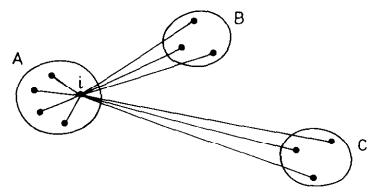
\includegraphics[scale=.6]{figures/silhouette_img.png}
	\caption{Illustration of the elements involved in the computation of the silhouette~\cite{rousseeuw1987silhouettes}.}
	\label{fig:silhouette}
\end{figure}

The function $b(i)$ is used to define the cluster neighbor of item $i$. This is likely the second best choice for object $i$. The function $b(i)$ depends on the availability of other clusters apart from $A$, so we have to assume that the number os clusters is greater than one.

Finally, the value of $s(i)$ is obtained by combining $a(i)$ and $b(i)$, as in  Equation~\ref{eq:s_i}:

\begin{equation} \label{eq:s_i}
s(i) = \frac{b(i) - a(i)}{max\{a(i), b(i)\}}
\end{equation}

When cluster $A$ contains only a single object it is unclear how $a(i)$ should be defined, and then in this case the value of $s(i)$ is set to zero. This choice is taken because
\begin{center}
	$-1 \le s(i) \le 1$
\end{center}

for each object $i$, and zero is the most neutral value. When $i$ is closer to 1, it implies that the object $i$ is "well-clustered", because the dissimilarity $a(i)$ is much smaller than the smallest "between" dissimilarity $b(i)$. On the other hand, when $i$ is closer to -1, it implies that $i$ has been "missclassified", because $a(i)$ is much larger than $b(i)$, and $i$ is closer to $B$ than $A$.

In summary, $s(i)$ measures how well object $i$ matches the clustering at hand, in other words, how well the item $i$ has been classified.


%%%%%%%%%%%%%%%%%%%

%S que tal trocarmos para approach .... afinal prometemos uma approach no titulo.

%\section{Methodology} \label{sec:methodology}

\section{Proposed Approach} \label{sec:methodology}

%S acho que aqui deveriamos descrever as caracterisitcas da abordagem, passos e introduzir esta seção e sua organizacao.
%Subdividi, vejam o que acham.

The proposed approach applies GE to generate clustering algorithms.......


\subsection{ Grammar Definition}

It includes a specific grammar, designed  using  Backus-Naur form. The grammar is as follows:




\begin{grammar}
	<GE> ::= <initialization> <distance> <command> 
	\\ <initialization> ::= "random" <k> | "uniform" <k>
	\\ <command> ::= <movement> | <movement> <command>
	\\ <movement> ::= "joinClusters" | "splitClusters" | "moveAverage" | "moveBetween" | "moveNear" 
	\\ <k> ::= "4" | "6" | "8" | "10" | "0"
	\\ <distance> ::= "eucledian" | "manhattan" | "chebyshev"
	\label{ge-clustering-grammar}
\end{grammar}


The first line specifies the main algorithm components: initialization, distance and command. 

For the initialization node two possibilities of terminal nodes were implemented: random and uniform. The random initialization randomly selects  objects as centroids of the clusters. The uniform initialization consists of finding the minimum and maximum values for each attribute of the dataset. This information is used to uniformly select the coordinates (within this range) for centroids. Moreover, for both initialization methods, an initial value of K (number of clusters) is chosen between five possible values: 4,6,8,10 and 0. If the chosen K value is equals to 0 it will be drawn a random number between 2 and 5. Note that, this K value is an initial value because the grammar allows to create or destroy clusters. 

In the case of the distance component, three possibilities of distance functions were implemented: \textit{Euclidean}, \textit{Manhattan} and \textit{Chebyshev}. The selected distance function will be used by all other functions that require information about the distance between data. 


%S o que é um programa infinito? nao existe este conceito, reescrever... 

The command component is the main body of the structure and it allows the creation or destruction of clusters as well as, movements of data from one cluster to other.  This component can potentially generate infinite programs since it has a recursion. In order to avoid the generation of infinite programs, a maximum depth value was setup to 20. The  terminal node is described at next.

\begin{itemize}
	\item JoinClusters: this terminal selects one random cluster, then computes the nearest cluster and merge both clusters.
	\item SplitClusters: this terminal searches for the cluster which has the highest average distance between the objects and its centroid and splits it. 
	\item MoveAverage:  this terminal gets one random object and calculates for each cluster the distance to all objects. The cluster whose average distance is the lowest will receive the selected object.
	\item MoveBetween: the terminal selects one random cluster and computes the nearest cluster. Then gets the object from the second cluster which has the lowest distance to the first centroid cluster and moves it.
	\item MoveNear:  the terminal gets one random object and calculates the distance to all clusters centroids. The cluster whose distance is the lowest between the centroid and the selected object will receive the object.
\end{itemize}

The designed grammar can generate clustering algorithms based on an integer vector as described on Subsection~\ref{subsection:grammaticalEvolution}. As example at next, this process is illustrated by beginning with the integer vector (genotype) and following the steps to decode into a clustering algorithm (phenotype). 

Supposing the following integer vector:

[199, 45, 172, 156, 157, 137, 191, 56, 27, 103, 5, 109, 81, 160, 124, 5, 182, 121, 247, 68, 180, 182, 100, 143, 141, 109]

The first gene is 199 and it is the entry point. The \textit{initialization} is the first non-terminal node. The next position in the vector is 45 and we have 2 options (\textit{random} and \textit{uniform}); thus 45 mod 2 will result in 1 which selects \textbf{uniform}. The initialization requires another selection for the initial K value. Following the vector, the next value is 172. There are 5 possibilities for K. Hence 172 mod 5 = 2, which is the index of the value \textbf{8}. The \textit{initialization} is ended. The second non-terminal node is \textit{distance}. There are three possible terminal node options. Next value in the vector is 156; 156 mod 3 results in 0, which corresponds to \textbf{Euclidean}. Now, it is necessary to decode the \textit{command} non-terminal node. Next position is 157 and two possibilities (\textit{movement} or \textit{movement + command}). Then 157 mod 2 = 1. Therefore, the selected one is \textbf{movement + command}. First step is to decode \textbf{movement} and the next step  is to  decode  \textbf{command}. Next position is 137 and there are 5 possibilities, thus the result is 2. The index 2 in the grammar is the \textbf{moveAverage} option. Now it is necessary to evaluate \textbf{command}; as before, there are 2 choices. As 191 mod 2 = 1, \textbf{movement + command} is selected again. This is repeated until the mod results 0,  and then, last \textbf{movement} is selected or until the max depth limit (20) is exceeded. The entire decoded clustering algorithm is presented in Algorithm~\ref{clustering-algoritm-example}.

\begin{algorithm}[!htb]
	\label{clustering-algoritm-example}
	Initialization initialization = new UniformInitialization(); \\
	DistanceFunction distanceFunction = new EucledianFunction(); \\
	int initialK = 8; \\
	boolean finished = false; \\
	int evaluations = 1000;\\
	ClusteringState 
	clusteringState = initialization.createInitialClusters(initialK); \\
	\While{!finished}{
		moveAverage(clusteringState); \\
		splitClusters(clusteringState); \\
		moveBetween(clusteringState); \\
		moveNear(clusteringState); \\
		joinClusters(clusteringState); \\
		joinClusters(clusteringState);\\
		
		finished = $!clusteringState.changed()$   $|| $		$evaluations>maxEvaluations$}{
		
	}
	\caption{Pseudo code from a decoded algorithm}
\end{algorithm}

The pseudo-code presented in Algorithm~\ref{clustering-algoritm-example} is an example that can be generated by the grammar. The stopping criterion in the generated algorithms is fixed using two conditions: first if no changes occurs in the clustering state or if the maximum number of evaluations exceeds. This can be seen at line 14 of the pseudo-code. The maximum number of evaluations was adjusted to 1000 after some experiments.


\subsection{Grammatical Evolution Process}

The next step of our approach is the grammatical evolution process which consists of evolving populations of integer vectors. To do this, we propose an algorithm called GE-Clust ({\it Grammatical Evolution of Clustering Algorithms}). GE-Clust individuals are converted to clustering algorithms and applied to a cluster dataset. In order to evaluate the individuals, a fitness function was designed and is presented in Equation~\ref{equation:fitness}.

\begin{align}
\label{equation:fitness}
fitness    &= \frac{\sum_{i=1}^e \frac{\sum_{j=1}^{p} s_{ij}}{p}}{e}
\
\end{align}

The $e$ value represents the number of independent executions of the clustering algorithm and was fixed to 10. The $p$ value is the number of objects of the respective dataset being used; $s_{ij}$ is the silhouette index (Sub-section~\ref{sec:sillhouetteIndex}) of the $j^{\text{th}}$ object of the $i^{\text{th}}$ execution. Basically the fitness function is given by the average of the silhouette value for every object of the dataset in each execution of the clustering algorithm.

%S estruturar a descrição do GE-Clust em itens: individual representation, operadores, fitness e caracteristicas do  evolution process.

GE-Clust, used to evolve the clustering algorithms, is similar to a traditional GA, however the individual solutions have not fixed length, whereas the generated algorithms can have different sizes. Since the solutions are not of fixed length it is possible after applying a crossover or mutation operator that one individual has less genes than the required for building a clustering algorithm. The approach for this situation is to continue getting the integer values from the beginning of the individual in order to fill all functions required by a clustering algorithm. Also, it is possible to occur the inverse situation: when an individual is bigger than the necessary to build a clustering algorithm. The strategy adopted here is to simply discard the portion that is not being used. It is worthwhile to mention that individuals in GE do not necessarily use all their genes to be decoded to a program. A prune operator was proposed by~\cite{ryan1998grammatical} to reduce the possibilities of crossover operations being applied on genes that are not decoded to a program. The prune operator consists on given a probability, truncate the offspring generated by the crossover and mutation operators. Another operator that was proposed to deal with GE is the duplication operator inspired by the biological background. It consists on duplicating a random number of genes in the end of the original individual, also given a probability of occurrence. The main idea here is to duplicate the genes in order to increase their presence on the overall individual.

The GE-Clust algorithm was implemented using the open source architecture from jMetal framework~\cite{jMetal}. jMetal is  easy to extend, has a well organized structure and also an active community.  

%%%%%%%%%%%%%%%%%%%%%%%%%%%%%%%%%%


\section{Experimental Evalution} \label{sec:experiments}

This section describes the experiments conducted to evaluate the proposed approach and the implemented algorithm GE-Clust.

\subsection{Experiment Setup}


The experiment used four well-known clustering datasets from UCI machine learning database~\cite{uci}. Table \ref{uci-experiments} shows the amount of instances, numbers of attributes and the data type of the datasets. 


\begin{table}[]
	\centering
	\caption{UCI datasets used in the experiments}
	\label{uci-experiments}
	\begin{tabular}{|l|l|l|l|l}
		\cline{1-4}
		\textbf{Dataset Name}                                           & \multicolumn{1}{l|}{\textbf{Intances}} & \multicolumn{1}{l|}{\textbf{Attributes}} & \textbf{Type}     \\ \hline
		\begin{tabular}[c]{@{}l@{}}Pima Indians\\ Diabetes\end{tabular} & 768                                    & 8                                        & Integer, Real     \\ \hline
		Stalog (Hearth)                                                 & 270                                    & 13                                       & Categorical, Real \\ \hline
		Iris                                                            & 150                                    & 4                                        & Real              \\ \hline
		\begin{tabular}[c]{@{}l@{}}Glass\\ Identification\end{tabular}  & 214                                    & 10                                       & Real              \\ \hline
	\end{tabular}
\end{table}



The GE-Clust was executed 10 independent runs with each dataset using the same configuration presented in Table~\ref{ge-configuration}. The evaluation of the individuals was made using the fitness function presented on Equation~\ref{equation:fitness}.

In order to make comparisons, the K-means algorithm was executed 10 times with different K values. The K value varied within the range 2 to 7 and only the best k configuration (the one whose obtained the highest fitness values) is considered.

\begin{table}[]
	\centering
	\caption{Configuration used in the GE-Clust}
	\label{ge-configuration}
	\begin{tabular}{|l|l|}
		\hline
		\textbf{Crossover  |  Probability}         & Single Point  | 0.95     \\ \hline
		\textbf{Mutation | Probability}            & Integer Mutation          |  0.10 \\ \hline
		\textbf{Prune  | Probability}      & Prune Operator           | 0.05   \\ \hline
		\textbf{Duplication Operator | Probability} & Duplication   | 0.05     \\ \hline
		\textbf{Population}                        & 100                               \\ \hline
		\textbf{Generations}                       & 200                               \\ \hline
	\end{tabular}
\end{table}

%S talvez seja melhor tb colocar um paragrafo sobre a metodologia de análise dos resultados.

\subsection{Results and Analysis}


%S será suficiente usar só  esta comparação com o fitness ??? não deveriamos usar outros indicadores?

Table \ref{results-ge-and-kmeans} presents the results obtained by both algorithms. The table contains average, 
standard deviation, minimum and maximum values of the fitness value,  from the best individual of each run of each algorithm. The amount of clusters (k) found by GE-Clust is also presented.



\begin{table*}[]
	\centering
	\caption{Results of GE-Clust best individual and also the fitness obtained by K-means algorithm}
	\label{results-ge-and-kmeans}
	\begin{tabular}{|c|c|c|c|c|c|}
		\hline
		\textbf{Dataset}           & \textbf{Algorithm} & \textbf{Statistics} & \textbf{Fitness} & \textbf{k}    & \textbf{Kruskal-Wallis Test}   \\ \hline
		\multirow{8}{*}{Pima Indians Diabetes} & \multirow{4}{*}{GE-Clust}           & Average                        & \textbf{0.605378}                    & 2                        & \multirow{8}{*}{TRUE} \\ \cline{3-5}
		&                               & Std Dev                        & 0.009389                    & 0                        &                       \\ \cline{3-5}
		&                               & Min                            & 0.586250                    & 2                        &                       \\ \cline{3-5}
		&                               & Max                            & 0.616885                   & 2                        &                       \\ \cline{2-5}
		& \multirow{4}{*}{K-Means}      & Average                        & 0.570102                   & \multirow{4}{*}{Fixed 2} &                       \\ \cline{3-4}
		&                               & Std Dev                        & 0,000000                   &                          &                       \\ \cline{3-4}
		&                               & Min                            & 0.570102                   &                          &                       \\ \cline{3-4}
		&                               & Max                            & 0.570102                   &                          &                       \\ \hline
		\multirow{8}{*}{Statlog (Heart)}       & \multirow{4}{*}{GE-Clust}           & Average                        & \textbf{0.597191}                    & 2                        & \multirow{8}{*}{TRUE} \\ \cline{3-5}
		&                               & Std Dev                        & 0.018334                    & 0                        &                       \\ \cline{3-5}
		&                               & Min                            & 0.384030                    & 2                        &                       \\ \cline{3-5}
		&                               & Max                            & 0.441919                     & 2                        &                       \\ \cline{2-5}
		& \multirow{4}{*}{K-Means}      & Average                        & 0.383325                    & \multirow{4}{*}{Fixed 2} &                       \\ \cline{3-4}
		&                               & Std Dev                        & 0.001524                    &                          &                       \\ \cline{3-4}
		&                               & Min                            & 0.382145                    &                          &                       \\ \cline{3-4}
		&                               & Max                            & 0.385096                    &                          &                       \\ \hline
		\multirow{8}{*}{Glass Identification}  & \multirow{4}{*}{GE-Clust}           & Average                        & 0.597191                    & 2                        & \multirow{8}{*}{TRUE} \\ \cline{3-5}
		&                               & Std Dev                        & 0.006850                    & 0                        &                       \\ \cline{3-5}
		&                               & Min                            & 0.588779                    & 2                        &                       \\ \cline{3-5}
		&                               & Max                            & 0.605818                    & 2                        &                       \\ \cline{2-5}
		& \multirow{4}{*}{K-Means}      & Average                        & \textbf{0.624822}                    & \multirow{4}{*}{Fixed 2} &                       \\ \cline{3-4}
		&                               & Std Dev                        & 0.000008                    &                          &                       \\ \cline{3-4}
		&                               & Min                            & 0.624818                    &                          &                       \\ \cline{3-4}
		&                               & Max                            & 0.624836                    &                          &                       \\ \hline
		\multirow{8}{*}{Iris}                  & \multirow{4}{*}{GE-Clust}           & Average                        & 0.644598                   & 2                        & \multirow{8}{*}{TRUE} \\ \cline{3-5}
		&                               & Std Dev                        & 0.013778                   & 0                        &                       \\ \cline{3-5}
		&                               & Min                            & 0.625916                   & 2                        &                       \\ \cline{3-5}
		&                               & Max                            & 0.674525                   & 2                        &                       \\ \cline{2-5}
		& \multirow{4}{*}{K-Means}      & Average                        & \textbf{0.681304}                   & \multirow{4}{*}{Fixed 2} &                       \\ \cline{3-4}
		&                               & Std Dev                        & 0.000000                   &                          &                       \\ \cline{3-4}
		&                               & Min                            & 0.681304                   &                          &                       \\ \cline{3-4}
		&                               & Max                            & 0.681304                   &                          &                       \\ \cline{3-4}							\hline
	\end{tabular}
\end{table*}

\begin{table*}[]
	\centering
	\caption{Statistics of algorithms execution time}
	\label{resultsTimeExecution}
	\begin{tabular}{|c|c|c|c|c|}
		\hline
		\textbf{Dataset}                       & \multicolumn{1}{l|}{\textbf{Statistics}} & \multicolumn{1}{l|}{\textbf{\begin{tabular}[c]{@{}l@{}}GE-Clust Execution\\ Time (h)\end{tabular}}} & \multicolumn{1}{l|}{\textbf{\begin{tabular}[c]{@{}l@{}}GE-Clust Best Individual \\ Execution Time (ms)\end{tabular}}} & \multicolumn{1}{l|}{\textbf{\begin{tabular}[c]{@{}l@{}}K-Means\\ Execution Time (ms)\end{tabular}}} \\ \hline
		\multirow{4}{*}{Pima Indians Diabetes}       & Average                                  & 261.7                                                  & 10581.7                                                                                                         & 
		102.6                                                                                               \\ \cline{2-5} 
		& Std Dev                                  & 56.5                                                                                       & 922.9                                                                                                           & 39.3                                                                                               \\ \cline{2-5} 
		& Min                                      & 199.0                                                                                         & 8809.9                                                                                                           & 71.0                                                                                                 \\ \cline{2-5} 
		& Max                                      & 349.0                                                                                        & 11933.0                                                                                                          & 71.0                                                                                                \\ \hline
		\multirow{4}{*}{Statlog (Heart)}       & Average                                  & 28.1                                                                                          & 1468.8                                                                                                          & 20.3                                                                                                \\ \cline{2-5} 
		& Std Dev                                  & 5.72                                                                                          & 243.5                                                                                                           & 11.6                                                                                                \\ \cline{2-5} 
		& Min                                      & 18.3                                                                                          & 885.0                                                                                                           & 7.0                                                                                                 \\ \cline{2-5} 
		& Max                                      & 35.7                                                                                          & 1738.0                                                                                                          & 52.0                                                                                                \\ \hline
		\multirow{4}{*}{Glass Identification}  & Average                                  & 9.0                                                                                          & 2602.1                                                                                                          & 14.8                                                                                                \\ \cline{2-5} 
		& Std Dev                                  & 2.6                                                                                           & 502.69                                                                                                          & 13.0                                                                                                \\ \cline{2-5} 
		& Min                                      & 5.5                                                                                          & 1610.0                                                                                                          & 3.0                                                                                                 \\ \cline{2-5} 
		& Max                                      & 12.9                                                                                          & 3185.0                                                                                                          & 45.0                                                                                                \\ \hline
		\multirow{4}{*}{Iris}                  & Average                                  & 7.2                                                                                           & 1074.5                                                                                                          & 15.1                                                                                                \\ \cline{2-5} 
		& Std Dev                                  & 2.7                                                                                           & 383.9                                                                                                           & 14.9                                                                                                \\ \cline{2-5} 
		& Min                                      & 4.1                                                                                           & 558.0                                                                                                           & 7.0                                                                                                 \\ \cline{2-5} 
		& Max                                      & 13.3                                                                                          & 1786.0                                                                                                          & 59.0                                                                                                \\ \hline
	\end{tabular}
\end{table*}



Looking at Table~\ref{results-ge-and-kmeans}, it is possible to observe that for the Pima Indian Diabetes, our approach reached 0.605 average of the fitness values obtained by the best individuals of 10 executions, while the K-means algorithm obtained a lower value equal to 0.570 on 10 executions.

%S referencia para o teste Kruskal

In the case of the Statlog (Heart) database,  the GE-Clust obtained a better average value of 0.409 while K-means algorithm reached 0.383. According to the  Kruskal-Wallis statistic test~\cite{}, these results have statistical difference.

In the Glass database, the results of GE-Clust have lower values than K-means, 0.597 and 0.624, respectively, also with statistical difference according to Kruskal- Wallis test. 

Finally, for the Glass database the best individuals of GE-Clust obtained 0.644 and the K-means reached 0.681, again with statistical difference.

Moreover, it is possible to note that for all 10 executions of the GE-Clust, the generated algorithms used two clusters. In the case of the k-means algorithm the results that presented the highest fitness values were obtained also using $k=2$. For the sake of space the results with $k = (3,4,5,6,7)$ were suppressed.

Table~\ref{resultsTimeExecution} presents some computational time information of the algorithms. The statistic summary of 10 GE-Clust executions, in hours, is presented in the third column. The fourth column shows the statistics related to the time taken, in milliseconds, to execute 10 times the best individual found by the GE-Clust. The fifth column presents the statistics related to the K-means algorithm execution.

By analysing the results it is possible to check our hypothesis and we can conclude that the clustering algorithms generated by our approach are able to reach good and acceptable values for the fitness function in terms of  the silhouette index. The fitness values obtained by the generated algorithms in two of four databases are better than the ones obtained by the K-means algorithm, although in the other databases the difference between the fitness values was very small. Therefore, in the context evaluated here, the generated algorithms proved to be competitive to K-means algorithm. Moreover, it is possible to highlight one advantage of the proposed approach: there is no need to configure the number of clusters which usually is a non-trivial task as mentioned by many authors~\cite{pham2005selection, yan2005methods, tibshirani2001estimating}.


\subsection{Threats to validity}

We identify the following points that can be threats to the validity of our results.
\begin{itemize}
	\item The parameters configuration was not tuned due to time constraints. The configuration was selected mainly based on literature works and some empirical experiments. It is possible that using a tuned configuration the results get improvements.
	\item The experiments were conducted using only 4 datasets: It is necessary to execute more experiments with a broader range of datasets in order to evaluate if the same behavior is maintained.
	\item The results strongly depend on the used grammar and future works should include new rules.
\end{itemize}



%%%%%%%%%%%%%%%%%%%%%%%%%%%%%%%%%%%%%%%%%%%%%%%%%%%%%%%

\section{Related Work} \label{sec:related_work}

In this section we describe some works that served as motivation and gave support to our work, and other ones that address the automatic generation of clustering algoritms.  

In~\cite{lourencco2012evolving,lourencco2015IEEE}, the authors proposed a Grammatical Evolution framework for the automatic design of Evolutionary Algorithms. The grammar defined has the ability to combine components that regularly appear in existing evolutionary algorithms, aiming to achieve novel and fully functional optimization methods. They used the Royal Road Functions to verify the capacity of the framework to evolve algorithms. The obtained results show that the framework is able to evolve simple evolutionary algorithms that can effectively solve the Royal Road instances. In some cases, unusual design solutions provided by the framework show competitive results with standard approaches.

The work of Miranda and Prud\^encio~\cite{miranda2015gefpso} was one of the papers used as base for this research. In the paper, the authors describe a framework to generate Particle Optimization Algorithm (PSO) using Grammatical Evolution. The paper details how to define the grammar (the production rules and expressions used), the map process using integer vector individuals, and how to use the grammar to generate the PSO algorithm. They performed experiments on the benchmark problems, and demonstrate that the proposed method generates useful designs which achieved competitive algorithms when compared to well succeeded algorithms from the literature.

In the paper~\cite{burke2012grammatical}, the authors note that GP approaches have been employed to automatically design constructive heuristics for solving problems. These algorithms reach results that are superior to that one obtained by human-created heuristics, but in general, they do not obtain results of same quality as local search heuristics. So in their research, they proposed the use of Grammatical Evolution to automatically generate good quality local search algorithms, that maintain their performance on new problem instances.

The paper of~\cite{bolton2015optimizing} is about the challenging task of projecting efficient algorithms for difficult combinatorial optimization problems. There is large amount of heuristic, meta-heuristic and hyper-heuristic methods showing that combining algorithms can produce better results than using each algorithm alone. In the paper, the authors propose the use of Genetic Programming to automate the design of Clustering algorithms. They create some functions that represents common operations made in clustering algorithms to represent the nodes required by GP, so the evolutionary could produce algorithms based on these functions. There are other approaches for the Clustering problem using GP like the paper of~\cite{boric2007genetic}, that uses Information Theoretic Fitness Measure -- a probabilistic interpretation of the space of objects -- for clustering.'

As we can observe, the automatic evolution of clustering algorithms is an important topic, which has been recently explored. Few works are dedicated to this subject.   Works in the literature are not based on Grammatical Evolution. They use other functions such as:  and, or and mathematical functions. The most similar work is the proposed in~\cite{bolton2015optimizing} but the paper does not have all the details needed to reply the study.  As far as we know this is the first time that Grammatical Evolution is used for clustering algorithm generation. 


%%%%%%%%%%%%%%%%%%%%%%%%%%%%%%%%%%%%%%%%%%%%%

\section{Conclusion}
\label{sec:conclusion}

In this study, the automatic design of clustering algorithms is faced by a Grammatical Evolution approach. Grammatical evolution is a form of genetic programming which uses a grammar to map between the genotype and the phenotype. The definition of a good rule set is crucial for the success of a GE approach. 

The proposed approach emcompasses i) a grammar,  projected for clustering algorithms, which uses common operations like moving or grouping objects; ii)  silhouette index, used as fitness function; and iii) the algorithm GE-Clust that implements the evolution process. 

A set of experiments were conducted using UCI databases. The results of the generated algorithms were compared to K-means. In 2 of 4 datasets the proposed approach reached best values, whit statistical difference, when compared with the K-means algorithm.

Based on the conducted experiments, it is possible to conclude that the proposed approach can generate useful clustering algorithms, capable to produce good solutions with respect to the silhouette index. Future works include to extend this study to other databases and the addition of other rules to the grammar with other important component for clustering algorithms.


%S acertar estas duas referencias: bolton e yan. o que são e de onde?

%Warning--empty journal in bolton2015optimizing
%Warning--empty year in bolton2015optimizing
%Warning--there's a number but no volume in langdon2013optimising
%Warning--empty journal in yan2005methods

%S ver o padrão de referencias do congresso, tem algumas que estão com iniciais somente, outras tem os nomes completos.
%S Tem referencia incompleta tb.

%Referências
\bibliographystyle{plain}
\bibliography{references}

% that's all folks
\end{document}


